\documentclass[11pt]{article}
\usepackage[utf8]{inputenc}
\usepackage[spanish]{babel}
\decimalpoint
\usepackage{amsmath}
\usepackage{amsthm}
\usepackage{amssymb}
\usepackage{graphicx}
\usepackage[margin=0.9in]{geometry}
\usepackage{fancyhdr}
\usepackage[inline]{enumitem}
\usepackage{float}
\usepackage{cancel}
\usepackage{bigints}
\usepackage{listings}
\usepackage{xcolor}
\usepackage{listingsutf8}
\usepackage{algpseudocode}
\usepackage{algorithm}
\usepackage{minted}
\pagestyle{fancy}
\setlength{\headheight}{15pt} 
\lhead{Práctica 7: Circuitos aritméticos}
\rhead{\thepage}
\lfoot{ESCOM-IPN}
\rfoot{Ontiveros Salazar Alan Enrique}
\renewcommand{\footrulewidth}{0.5pt}
\setlength{\parskip}{0.5em}
\newcommand{\ve}[1]{\overrightarrow{#1}}
\newcommand{\abs}[1]{\left\lvert #1 \right\lvert}
\date{9 de octubre de 2017}
\title{Práctica 7: Circuitos aritméticos}
\author{2CM2}

\begin{document}
		\begin{titlepage}
			\begin{center}
				
				% Upper part of the page. The '~' is needed because \\
				% only works if a paragraph has started.
				
				\noindent
				\begin{minipage}{0.5\textwidth}
					\begin{flushleft} \large
						\includegraphics[width=0.3\textwidth]{../ipn.png}
					\end{flushleft}
				\end{minipage}%
				\begin{minipage}{0.55\textwidth}
					\begin{flushright} \large
						\includegraphics[width=0.7\textwidth]{../escom.png}
					\end{flushright}
				\end{minipage}
				
				\textsc{\LARGE Instituto Politécnico Nacional}\\[0.5cm]
				
				\textsc{\Large Escuela Superior de Cómputo}\\[1cm]
				
				% Title
				
				{ \huge Práctica 7: Circuitos aritméticos \\[1cm] }
				
				{ \Large Unidad de aprendizaje: Fundamentos de diseño digital} \\[1cm]
				
				{ \Large Grupo: 2CM2 } \\[1cm]
				
				\noindent
				\begin{minipage}{0.5\textwidth}
					\begin{flushleft} \large
						\emph{Alumnos:}\\
						López Manríquez Ángel\\
						Ontiveros Salazar Alan Enrique\\
						Rosas Hernández Óscar Andrés
					\end{flushleft}
				\end{minipage}%
				\begin{minipage}{0.5\textwidth}
					\begin{flushright} \large
						\emph{Profesor:} \\
						Aguilar Sánchez Fernando
					\end{flushright}
				\end{minipage}
				
				\vfill
				
				% Bottom of the page
				{\large 9 de octubre de 2017}
			\end{center}
		\end{titlepage}
	
	\maketitle
	
	\section{Código VHDL}
	\subsection{Medio sumador}
	\inputminted[tabsize=4,breaklines,linenos]{vhdl}{halfAdder.vhd}
	
	\subsection{Sumador completo}
	\inputminted[tabsize=4,breaklines,linenos]{vhdl}{fullAdder.vhd}
	
	\subsection{Medio restador}
	\inputminted[tabsize=4,breaklines,linenos]{vhdl}{halfSubtractor.vhd}
	
	\subsection{Restador completo}
	\inputminted[tabsize=4,breaklines,linenos]{vhdl}{fullSubtractor.vhd}
	
	\subsection{Sumador de 4 bits}
	\inputminted[tabsize=4,breaklines,linenos]{vhdl}{fourBitsAdder.vhd}
	
	\clearpage
	
	\section{Reporte de pines}
	\subsection{Medio sumador}
	\inputminted[tabsize=4,breaklines,linenos]{vhdl}{halfAdder.rpt}
	
	\subsection{Sumador completo}
	\inputminted[tabsize=4,breaklines,linenos]{vhdl}{fullAdder.rpt}
	
	\subsection{Medio restador}
	\inputminted[tabsize=4,breaklines,linenos]{vhdl}{halfSubtractor.rpt}
	
	\subsection{Restador completo}
	\inputminted[tabsize=4,breaklines,linenos]{vhdl}{fullSubtractor.rpt}
	
	\subsection{Sumador de 4 bits}
	\inputminted[tabsize=4,breaklines,linenos]{vhdl}{fourBitsAdder.rpt}
	
	\section{Tabla de verdad}
	\subsection{Medio sumador}
	\begin{table}[H]
	    \centering
	    \begin{tabular}{|c|c|c|c|c|}
	         \hline
	         $a$ & $b$ & & $c$ & $s$ \\ \hline
	         0 & 0 & & 0 & 0 \\ \hline
	         0 & 1 & & 0 & 1 \\ \hline
	         1 & 0 & & 0 & 1 \\ \hline
	         1 & 1 & & 1 & 0 \\ \hline
	    \end{tabular}
	\end{table}
	
	\subsection{Sumador completo}
	\begin{table}[H]
	    \centering
	    \begin{tabular}{|c|c|c|c|c|c|}
	         \hline
	         $a$ & $b$ & $c_{in}$ & & $c_{out}$ & $s$ \\ \hline
	         0 & 0 & 0 & & 0 & 0 \\ \hline
	         0 & 0 & 1 & & 0 & 1 \\ \hline
	         0 & 1 & 0 & & 0 & 1 \\ \hline
	         0 & 1 & 1 & & 1 & 0 \\ \hline
	         1 & 0 & 0 & & 0 & 1 \\ \hline
	         1 & 0 & 1 & & 1 & 0 \\ \hline
	         1 & 1 & 0 & & 1 & 0 \\ \hline
	         1 & 1 & 1 & & 1 & 1 \\ \hline
	    \end{tabular}
	\end{table}
	
	\subsection{Medio restador}
	\begin{table}[H]
	    \centering
	    \begin{tabular}{|c|c|c|c|c|}
	         \hline
	         $x$ & $y$ & & $b$ & $r$ \\ \hline
	         0 & 0 & & 0 & 0 \\ \hline
	         0 & 1 & & 1 & 1 \\ \hline
	         1 & 0 & & 0 & 1 \\ \hline
	         1 & 1 & & 0 & 0 \\ \hline
	    \end{tabular}
	\end{table}
	
	\subsection{Restador completo}
	\begin{table}[H]
	    \centering
	    \begin{tabular}{|c|c|c|c|c|c|}
	         \hline
	         $x$ & $y$ & $b_{in}$ & & $b_{out}$ & $r$ \\ \hline
	         0 & 0 & 0 & & 0 & 0 \\ \hline
	         0 & 0 & 1 & & 1 & 1 \\ \hline
	         0 & 1 & 0 & & 1 & 1 \\ \hline
	         0 & 1 & 1 & & 1 & 0 \\ \hline
	         1 & 0 & 0 & & 0 & 1 \\ \hline
	         1 & 0 & 1 & & 0 & 0 \\ \hline
	         1 & 1 & 0 & & 0 & 0 \\ \hline
	         1 & 1 & 1 & & 1 & 1 \\ \hline
	    \end{tabular}
	\end{table}
	
	\section{Circuito lógico}
	\subsection{Medio sumador}
	\begin{figure}[H]
		\centering
		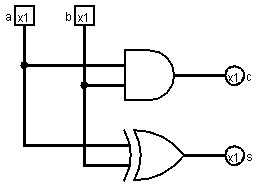
\includegraphics[scale=0.7]{halfAdder.png}
	\end{figure}
	
	\subsection{Sumador completo}
	\begin{figure}[H]
		\centering
		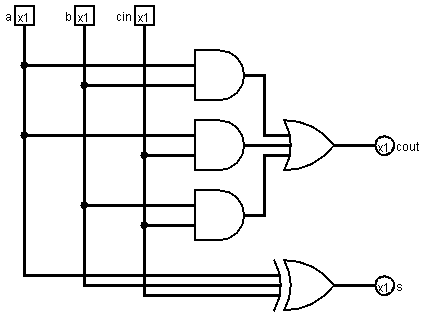
\includegraphics[scale=0.7]{fullAdder.png}
	\end{figure}
	
	\subsection{Medio restador}
	\begin{figure}[H]
		\centering
		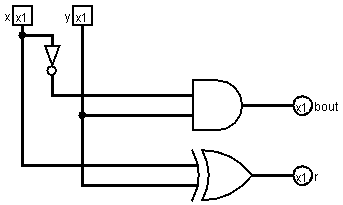
\includegraphics[scale=0.7]{halfSubtracter.png}
	\end{figure}
	
	\subsection{Restador completo}
	\begin{figure}[H]
		\centering
		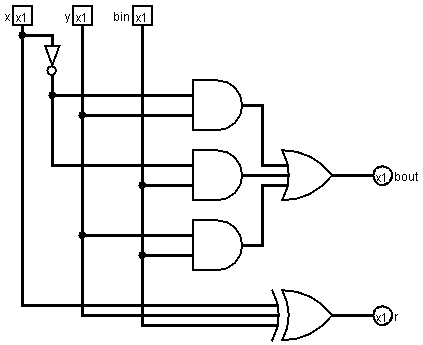
\includegraphics[scale=0.7]{fullSubtracter.png}
	\end{figure}
	
	\section{Circuito armado}
	\begin{figure}[H]
		\centering
		\includegraphics[scale=0.17]{../circuito2.jpg}
	\end{figure}
	
\end{document}